\subsection{Introduction}
\begin{frame}
    \small
    \begin{columns}
	\begin{column}
	    {0.75\textwidth}
            %{\color{darkblue}New generation of Transition Metal ECPs}\\
            For accurate calculations of functional materials (e.g. perovskites), explicitly correlated methods like QMC need to be solving the {\em correct} Hamiltonian. \\
            \bigskip 
            Effective Core Potentials (ECPs) are necessary in order to feasibly tackle large systems, include relativity, etc.\\
	\end{column}
	\begin{column}
	    {0.25\textwidth}
	    \begin{figure}[h]
		\centering
		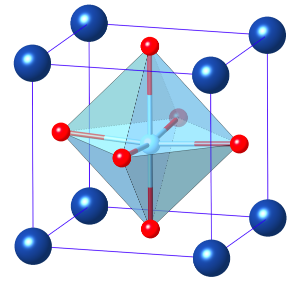
\includegraphics[width=0.75\textwidth]{figures/material}
	    \end{figure}
	\end{column}
    \end{columns}
    \bigskip
  \color{ForestGreen}
  We envision constructing a new generation of pseudopotentials that are highly accurate and isospectral to the original many-body Hamiltonian:
  \begin{itemize}
    \item<2->[$\rightarrow$] \color{ForestGreen}{\underline{Many-body construction}.} \color{black}{Constructed from relativistic {\it many-body} spectra leading to the reproduction of {\it nearly exact} many-body properties.}
    \item<3->[$\rightarrow$] \color{ForestGreen}{\underline{Reliable and universal}.} \color{black}{Tested and validated in many-body framework. Usable in both mean-field and many-body methods (in the spirit of the original all-electron $H$)}
 %   \item<4>[$\rightarrow$] \color{ForestGreen}{\underline{Simple and compact}.} \color{black}{As a first attempt, we try to use a form that is as simple as possible and find its accuracy limits}
  \end{itemize}
    
\end{frame}

\subsection{ECP Parametrization}
\begin{frame}
    \begin{block}
	{ECP Parametrization}
	We choose a semi-local parametrization for the ECPs.\\ 
    \end{block}
    \begin{center}
        \begin{tcolorbox}[enhanced,drop lifted shadow,boxrule=0.1pt,colback=blue!15,width=0.41\textwidth]
            $H_{\rm val} = \sum\limits_i \left[ T_i^{\rm kin}+ V_i^{\rm pp} \right] +  \sum\limits_{i<j}\frac{1}{r_{ij}}$
        \end{tcolorbox}
    \end{center}
    where 
    \begin{equation*}
	V_i^{\rm pp} = V_{\rm loc}(r_i) + \sum\limits_{\ell = 0} V_{\ell}(r_i) | \ell m \rangle \langle \ell m |, \quad V_\ell(r) = \sum_{k=1} \beta_{\ell k} e^{-\alpha_{\ell k}r^2}
    \end{equation*}
    and the local channel is finite at the origin
    \begin{equation*}
	V_{\rm loc}(r) = -\frac{Z_{\rm eff}}{r}\left( 1-e^{-\alpha r^2} \right) + \alpha Z_{\rm eff} r e^{-\beta r^2} + \sum_{k=1} \gamma_k e^{-\delta_i r^2}
    \end{equation*}
\end{frame}

\subsection{ECP Construction}
\begin{frame}
    {\color{ForestGreen}Many-body spectra and norm-conservation}
    \begin{itemize}
        \item Total Objective Function: \\
            $ \mathcal{O}^2 = \omega_0 \mathcal{E}^2 + \omega_1 \mathcal{N}^2 $, where $\omega_0,\omega_1$ are tunable weights\\
        \item CCSD(T) energy consistency:\\
            $\mathcal{E}^2 = \sum_s \left( \Delta E_s^{\rm ECP } -\Delta E_s^{\rm AE} \right)^2$, note that $\Delta E_s^{\rm AE}$ agrees with experiment to $\le 0.03$~eV
        \item Norm-conservation: \\
        $\mathcal{N}^2 = \sum_\ell\left( N_\ell^{\rm ECP}-N_\ell^{\rm AE} \right)^2 + \left(V_\ell^{\rm ECP} - V_\ell^{\rm AE}\right)^2 + \left(S_\ell^{\rm ECP}-S_\ell^{\rm AE}\right)^2 + \left( \epsilon_\ell^{\rm ECP} - \epsilon_\ell^{\rm AE} \right)^2$ where \\
        $N_\ell$: norm inside cutoff radius, $V_\ell, S_\ell, \epsilon_\ell$: value, derivative, eigenvalue of the orbital
    \end{itemize}
\end{frame}

\subsection{Main Group Elements}
\begin{frame}

  \large

  {\color{NavyBlue}Discrepancies from AE atomic spectrum \& CCSD(T) binding curve: }%{\color{RedOrange}\quad$\sum_s\big(\Delta E_s^{ECP}-\Delta E_s^{AE}\big)^2$}}

%  \bigskip
%  {\color{ForestGreen} CCSD(T) and Spectral  optimization: } \only<2>{{\color{red} (with FC)}}

  \only<1-1>{
  \begin{columns}
    \begin{column}{0.5\textwidth}
    \vfill
    \centering
    {\Large \color{blue}{O Atomic Spectrum (eV)} }
    \bigskip
     
    \small
    \begin{tabular}{lrrc}
     \hline
     \hline
     Core Approx. & $\Delta$IP(I) & $\Delta$EA & MAD \\
     \hline
     UC          & $ -0.0142 $ & $ -0.0017 $ & $ 0.0865 $ \\  
     BFD         & $ -0.0438 $ & $ -0.0105 $ & $ 0.3275 $ \\ 
     TN-DF       & $ -0.0436 $ & $ -0.0092 $ & $ 0.2669 $ \\
     TN-CEPP     & $ -0.0192 $ & $ -0.0259 $ & $ 0.1442 $ \\
     TN-eCEPP    & $ -0.0053 $ & $  0.0083 $ & $ 0.1434 $ \\
     \hline
     Spectral    & $ -0.0058 $ & $ -0.0044 $ & $ 0.0078 $ \\
     Spatial     & $ -0.0118 $ & $  0.0012 $ & $ 0.1303 $ \\
     Spec/Space  & $  0.0083 $ & $  0.0036 $ & $ 0.0192 $ \\
     \hline
     \hline
    \end{tabular}
    \end{column}
    \begin{column}{0.5\textwidth}
      \begin{figure}
        \centering
        \vspace*{-0.05\textheight}
        \begin{tikzpicture}
          \node[inner sep=0] at (0,0) {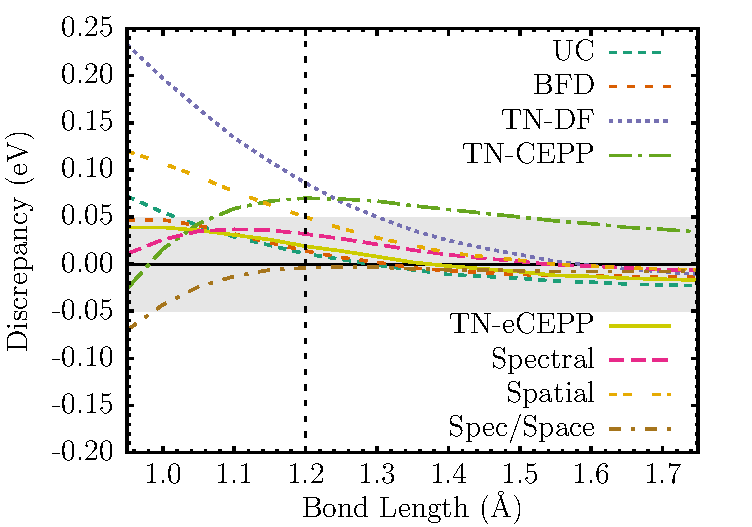
\includegraphics[width=\textwidth]{figures/o2_all_diffs}};
          \node at (0,3.0) {\Large \color{blue}{O$_2(^3\Sigma_g)$} };
          \draw[red, thick, ->] (-2.65,-2.65) node[anchor=north] {\tiny Near Dissociation Threshold} (-2.5,-2.75)  -- (-2.5,-2.3);
          \draw[red, thick, ->] (0,2) node[anchor=west] (0.6,0) {\tiny All-electron $R_0$} -- (-0.5,2);
        \end{tikzpicture}
      \end{figure}
    \end{column}
  \end{columns}
  }
  \only<2-2>{
  \begin{columns}
    \begin{column}{0.5\textwidth}
    \vfill
    \centering
    {\Large \color{blue}{O Atomic Spectrum (eV)} }
    \bigskip
     
    \small
    \begin{tabular}{lrrc}
     \hline
     \hline
     Core Approx. & $\Delta$IP(I) & $\Delta$EA & MAD \\
     \hline
     UC          & $ -0.0142 $ & $ -0.0017 $ & $ 0.0865 $ \\  
     BFD         & $ -0.0438 $ & $ -0.0105 $ & $ 0.3275 $ \\ 
     TN-DF       & $ -0.0436 $ & $ -0.0092 $ & $ 0.2669 $ \\
     TN-CEPP     & $ -0.0192 $ & $ -0.0259 $ & $ 0.1442 $ \\
     TN-eCEPP    & $ -0.0053 $ & $  0.0083 $ & $ 0.1434 $ \\
     \hline
     \color{darkblue} Spectral    & \color{darkblue}$ -0.0058 $ & \color{darkblue}$ -0.0044 $ & \color{darkblue}$ 0.0078 $ \\
     Spatial     & $ -0.0118 $ & $  0.0012 $ & $ 0.1303 $ \\
     Spec/Space  & $  0.0083 $ & $  0.0036 $ & $ 0.0192 $ \\
     \hline
     \hline
    \end{tabular}
    \end{column}
    \begin{column}{0.5\textwidth}
      \begin{figure}
        \centering
        \vspace*{-0.05\textheight}
        \begin{tikzpicture}
          \node[inner sep=0] at (0,0) {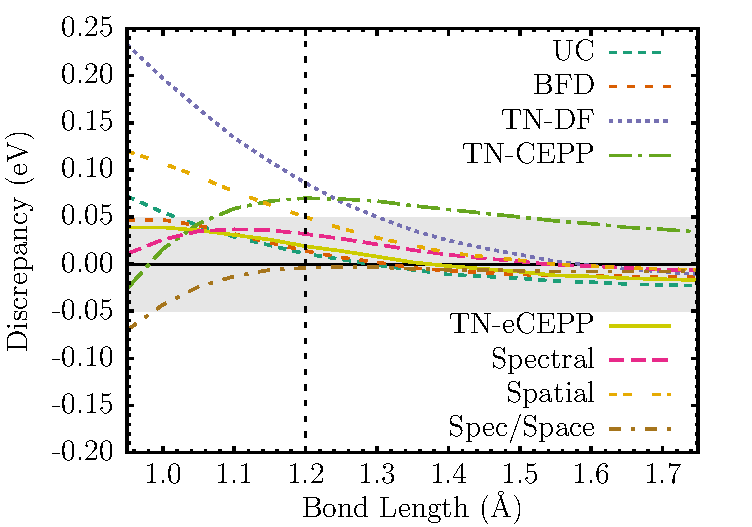
\includegraphics[width=\textwidth]{figures/o2_all_diffs}};
          \node at (0,3.0) {\Large \color{blue}{O$_2(^3\Sigma_g)$} };
          \draw[red, thick, ->] (-2.65,-2.65) node[anchor=north] {\tiny Near Dissociation Threshold} (-2.5,-2.75)  -- (-2.5,-2.3);
          \draw[red, thick, ->] (0,2) node[anchor=west] (0.6,0) {\tiny All-electron $R_0$} -- (-0.5,2);
        \end{tikzpicture}
      \end{figure}
    \end{column}
  \end{columns}
  }
\end{frame}

\begin{frame}

  \large

  \onslide<1->{\color{NavyBlue}Transferability Testing}
\begin{figure}
  \color{black}
  \centering
  \subfloat{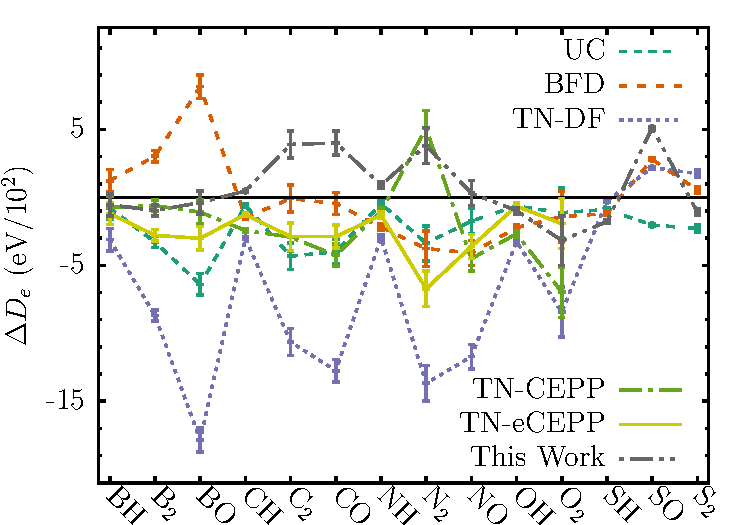
\includegraphics[height=0.45\textheight,width=0.33\textwidth]{figures/de.pdf}}
  \subfloat{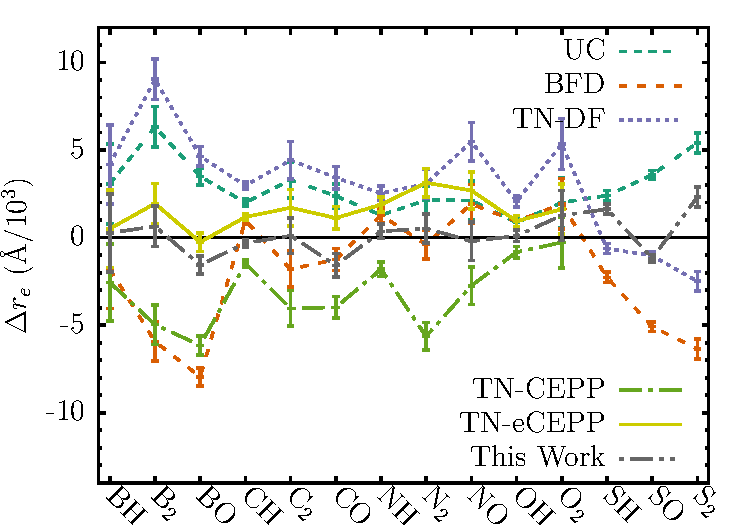
\includegraphics[height=0.45\textheight,width=0.33\textwidth]{figures/re.pdf}}
  \subfloat{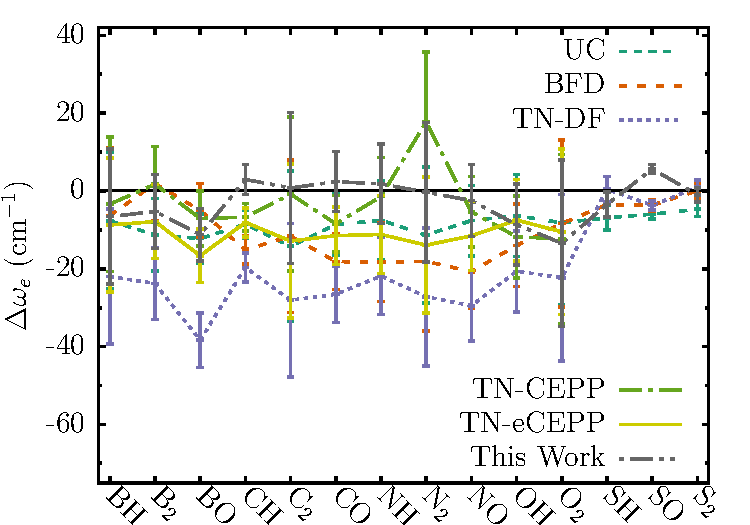
\includegraphics[height=0.45\textheight,width=0.33\textwidth]{figures/we.pdf}}
\end{figure}

\small
\centering
\color{black}
    \begin{tabular}{c | cccccc}
	\hline
	\hline
	       MAD   &   UC  &   BFD  &    TN-DF &   TN-CEPP &  TN-eCEPP &   This Work \\
	\hline
	 $D_e$    (  eV/$10^2$)     &    {\color{ForestGreen}\bf 2.0(2)} &     6.9(2) &     2.3(2) &     2.9(3) &     2.6(3) &   {\color{ForestGreen}\bf 2.0(2)}   \\
	 $r_e$      (\AA/$10^3$)    &    2.9(3) &     2.8(3) &     3.7(3) &     3.1(3) &     1.5(3) &   {\color{ForestGreen}\bf 0.9(3)}   \\
	 $\omega_e$ (cm$^{-1}$)     &      9(3) &      10(3) &      20(3) &       7(4) &      11(4) &     {\color{ForestGreen}\bf 5(3)}   \\
	 $D_{diss}$      (eV/$10^2$)      &    13.10 &      19.96 &     11.75  &     20.94   &     7.79 &       {\color{ForestGreen}\bf 5.75} \\
	 \hline
	 \hline
    \end{tabular}

\end{frame}

\subsection{Transition Metals}
\begin{frame}
    \begin{columns}
	\begin{column}
	    {0.5\textwidth}
	    \begin{itemize}
		\footnotesize
	        \item[] {\bf AE Reference:} RCCSD(T) correlating {\em all} electrons\\
		\item[] {\color[HTML]{E41A1C} \bf UC:} is a uncorrelated Ne-core RCCSD(T)  \\
		\item[] {\color[HTML]{377EB8} \bf BFD:} Burkatzki-Filippi-Dolg DHF ECPs for QMC\\
		        {\color[HTML]{4DAF4A} \bf  STU:} Stuttgart group DHF ECPs\\
			{\color[HTML]{984EA3} \bf TN17:} Trail-Needs correlated ECPs for QMC \\
			{\color[HTML]{FF7F00} \bf Our ccECP:} Our correlation-consistent ECP
		\item[]
		\item[] {\color{wolfred} \bf Discrepancy:} \\
		    \begin{tcolorbox}[enhanced,drop lifted shadow,boxrule=.1pt,colback=blue!15,width=0.75\textwidth]
			    \centering
	        	    $\left(E_{s}^{\rm ECP}-E_{\rm GS}^{\rm ECP}\right) - \left( E_{s}^{\rm AE} - E_{\rm GS}^{\rm AE} \right) $
	        	\end{tcolorbox}
	    \end{itemize}
	\end{column}
	\begin{column}
	    {0.55\textwidth}
	    \only<1-1>{
   	   	 \begin{figure}[h]
   	   	     \centering
	   	     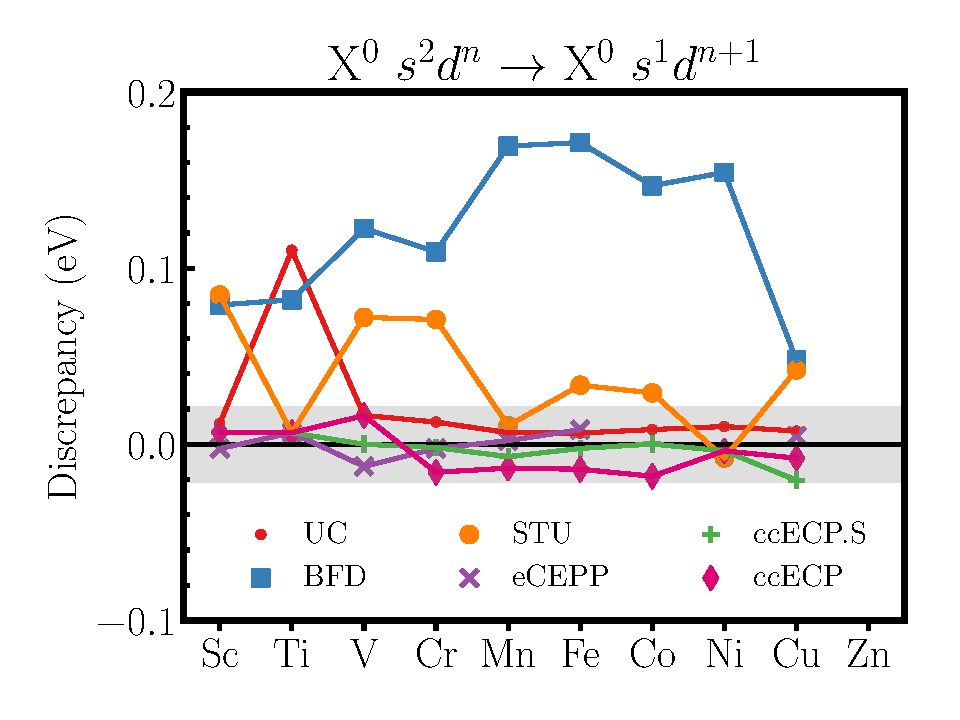
\includegraphics[width=\textwidth]{figures/Is2dn_to_Is1dn1}
   	   	 \end{figure}
	    }
	    %\only<2-2>{
   	    %    \begin{figure}[h]
   	    %        \centering
	    %        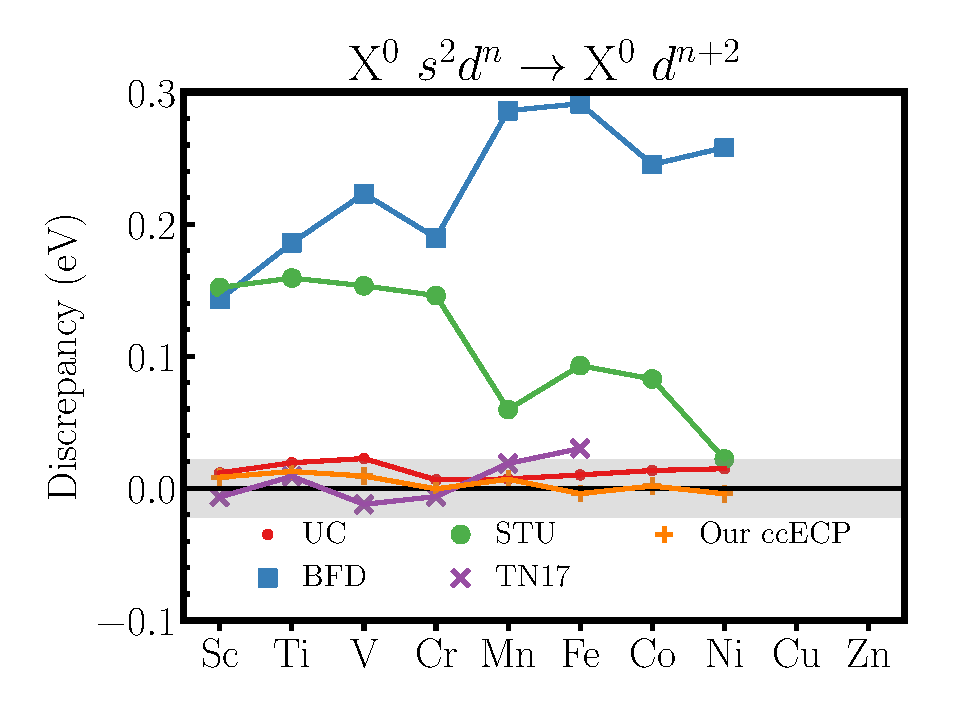
\includegraphics[width=\textwidth]{figures/Is2dn_to_Idn2}
   	    %    \end{figure}
	    %}
	    %\only<3-3>{
   	    %    \begin{figure}[h]
   	    %        \centering
	    %        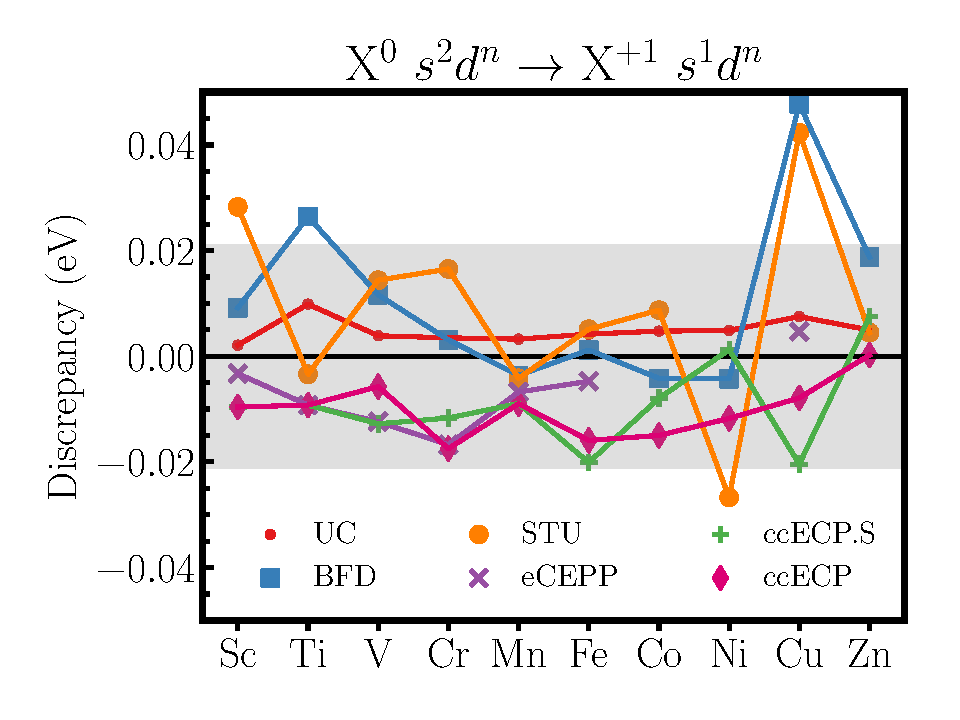
\includegraphics[width=\textwidth]{figures/Is2dn_to_IIs1dn}
   	    %    \end{figure}
	    %}
	    %\only<4-4>{
   	    %    \begin{figure}[h]
   	    %        \centering
	    %        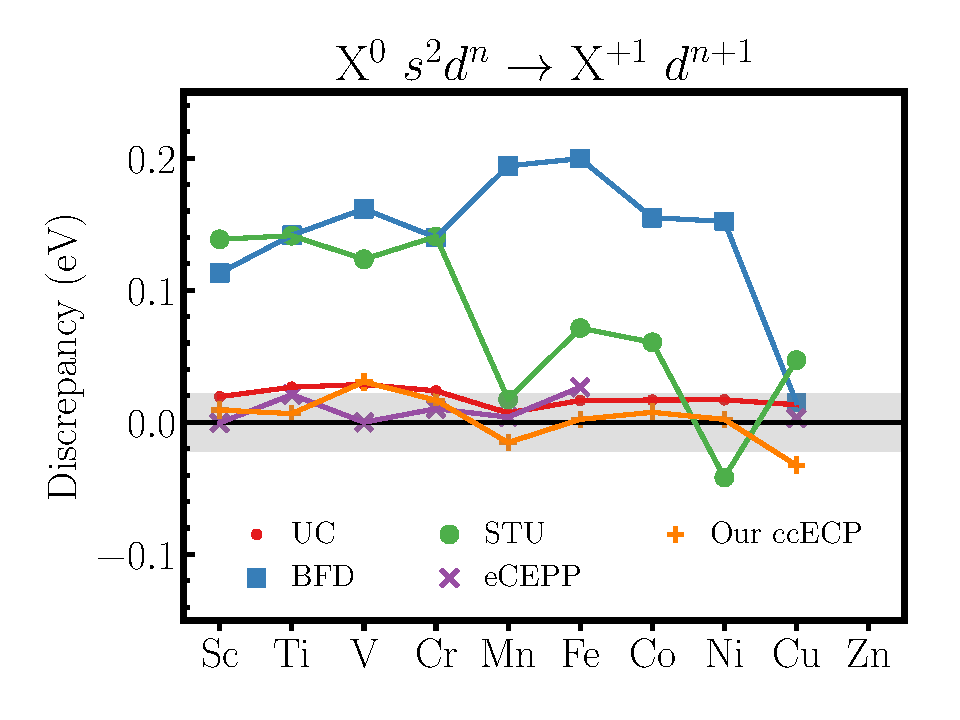
\includegraphics[width=\textwidth]{figures/Is2dn_to_IIdn1}
   	    %    \end{figure}
	    %}
	    %\only<5-5>{
   	    %    \begin{figure}[h]
   	    %        \centering
	    %        \includegraphics[width=\textwidth]{figures/ea}
   	    %    \end{figure}
	    %}
	    \only<2-2>{
   	        \begin{figure}[h]
   	            \centering
	            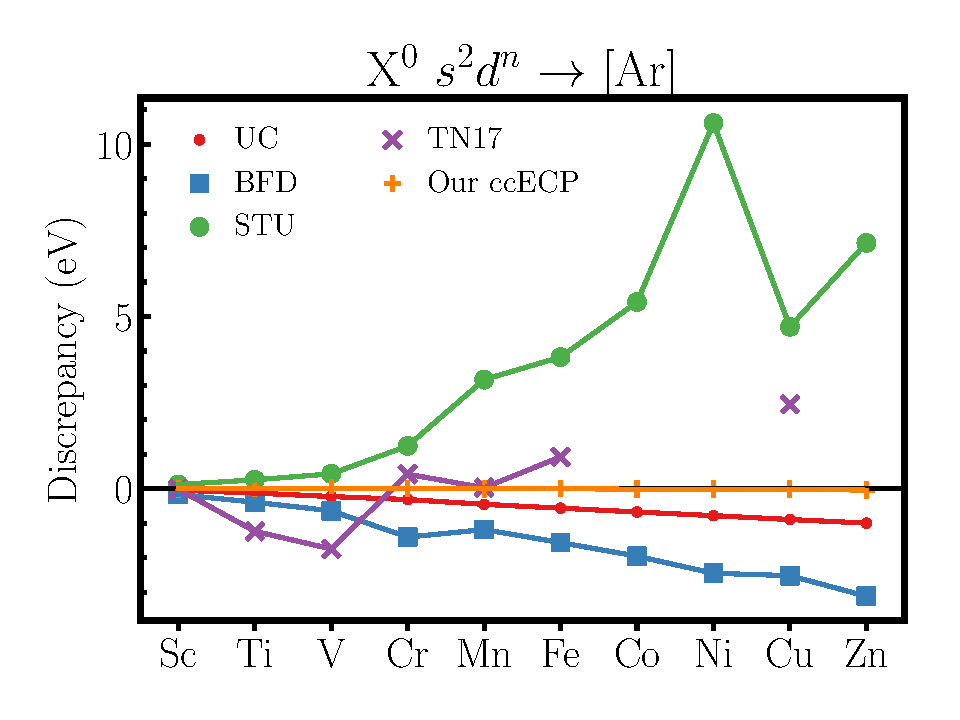
\includegraphics[width=\textwidth]{figures/ar}
   	        \end{figure}
	    }
	\end{column}
    \end{columns}
\end{frame}

\begin{frame}
    \begin{columns}
	\begin{column}
	    {0.45\textwidth}
	    \begin{block}
		{Example Spectrum (Ni)}
                \begin{table}
		    \scriptsize
                \centering
                \begin{tabular}{ll|ll}
		{[Ar] $3d^84s^2$ }  & $^3F$ &  {[Ar] $3d^5$ }      & $^6S$\\
                {[Ar] $3d^94s^1$ }  & $^3D$ &  {[Ar] $3d^4$ }      & $^5D$\\ 
                {[Ar] $3d^{10}$ }   & $^1S$ &  {[Ar] $3d^3$ }      & $^4F$\\
                {[Ar] $3d^84s^1$ }  & $^4F$ &  {[Ar] $3d^2$ }      & $^3F$\\
                {[Ar] $3d^9$ }      & $^2D$ &  {[Ar] $3d^1$ }      & $^2D$\\
                {[Ar] $3d^8$ }      & $^3F$ &  {[Ar] }             & $^1S$\\
                {[Ar] $3d^7$ }      & $^4F$ &  {[Ne] $3s^2$ }      & $^1S$\\
                {[Ar] $3d^6$ }      & $^5D$ &  {[Ar] $3d^94s^2$ }  & $^2D$\\
                \end{tabular}
                \end{table}
	    \end{block}
	    {\color{wolfred}Mean Absolute Deviation:}
	    \small{
		\begin{tcolorbox}[enhanced,drop lifted shadow,boxrule=0.1pt,colback=blue!15]
		    $\frac{1}{N}\sum\limits_{s=1}^N \left| \left( E_s^{\rm PP}-E_{\rm GS}^{\rm PP} \right) - \left( E_s^{\rm AE}-E_{GS}^{\rm AE} \right)\right| $
	        \end{tcolorbox}
	    }
	\end{column}
	\begin{column}
	    {0.55\textwidth}
   	     \begin{figure}[h]
   	         \centering
		 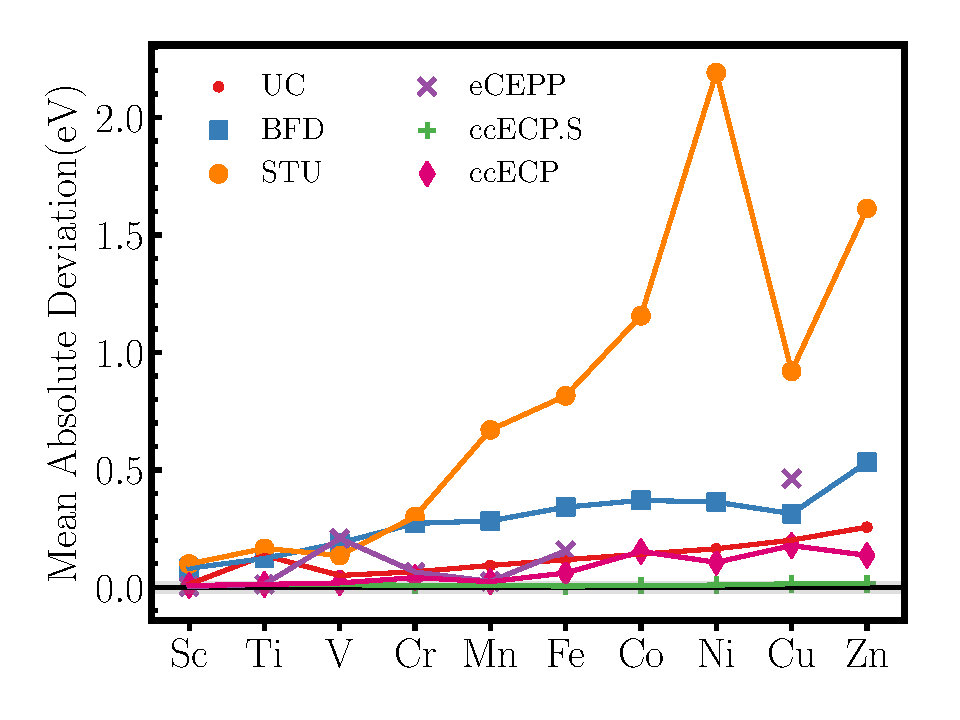
\includegraphics[width=\textwidth]{figures/mad}
   	     \end{figure}
	\end{column}
    \end{columns}
\end{frame}

\subsection{Transferability with Selected Molecules}

\begin{frame}
    \begin{center}
	{\Large\color{wolfred}{\bf Monoxides}}
    \end{center}
    \begin{columns}
	\begin{column}
	    {0.5\textwidth}
	    \begin{figure}[h]
		\centering
		\caption*{ScO binding curve discrepancies}
		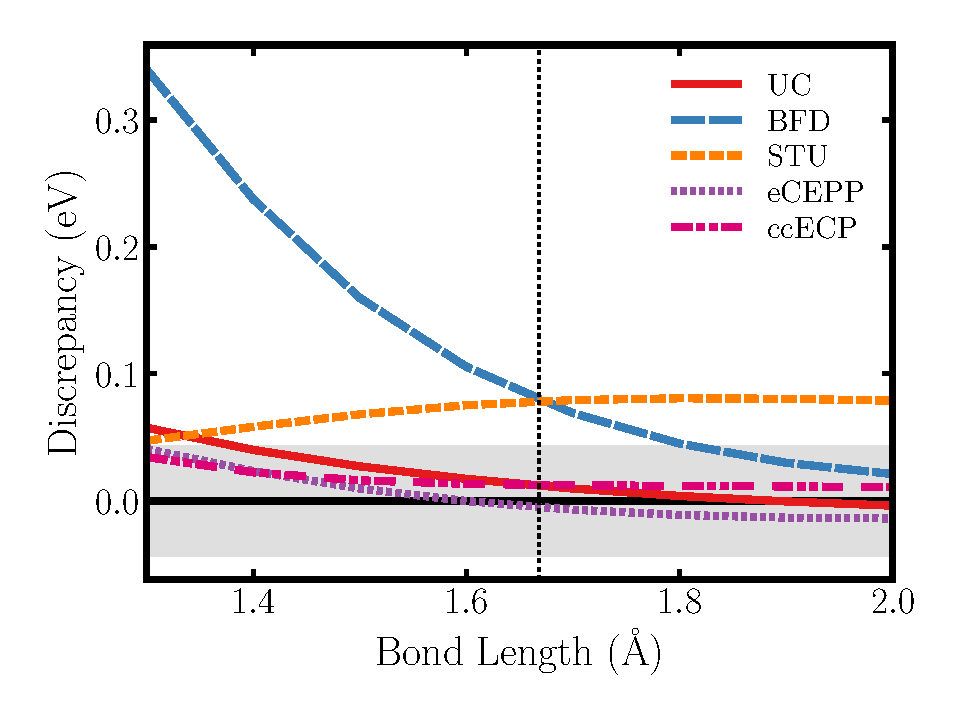
\includegraphics[width=\textwidth]{figures/ScO}
	    \end{figure}
	\end{column}
	\begin{column}
	    {0.5\textwidth}
	    \begin{figure}[h]
		\centering
		\caption*{VO binding curve discrepancies}
		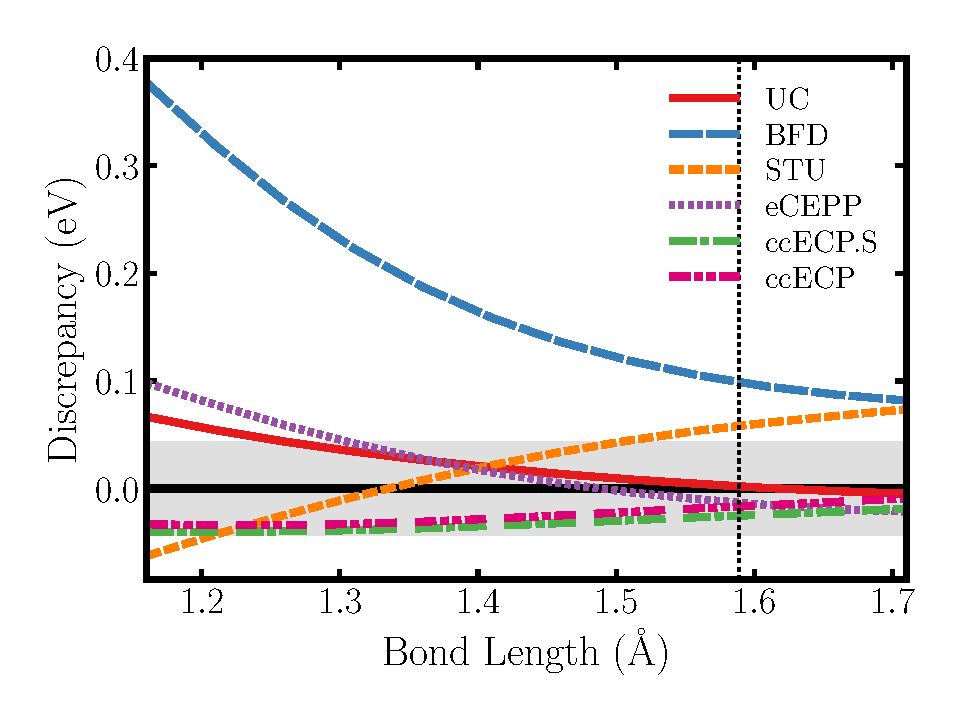
\includegraphics[width=\textwidth]{figures/VO}
	    \end{figure}
	\end{column}
    \end{columns}
\end{frame}

